\documentclass[tikz]{standalone}

\begin{document}
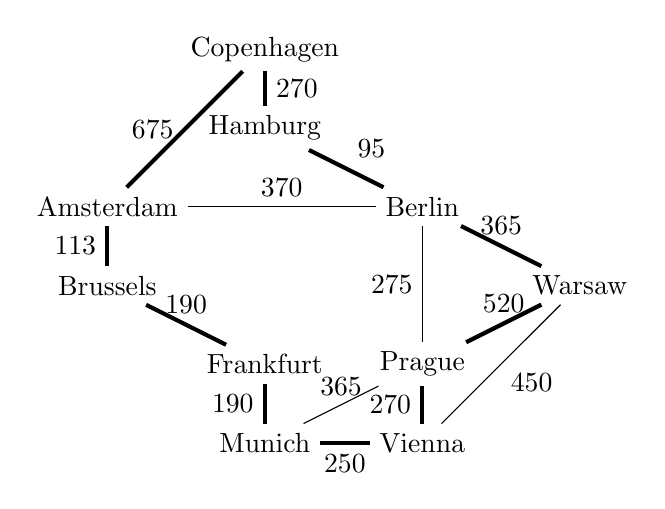
\begin{tikzpicture}
\path(0,0) node(Amsterdam){Amsterdam} (2,1) node(Hamburg){Hamburg} (4,0) node(Berlin){Berlin} (2,2) node(Copenhagen){Copenhagen} (0,-1) node(Brussels){Brussels} (6,-1) node(Warsaw){Warsaw} (2,-2) node(Frankfurt){Frankfurt} (4,-2) node(Prague){Prague} (2,-3) node(Munich){Munich} (4,-3) node(Vienna){Vienna};

\draw[line width=1.5pt] (Amsterdam) -- node[left]{675} (Copenhagen);
\draw (Amsterdam) -- node[above]{370} (Berlin);
\draw[line width=1.5pt] (Amsterdam) -- node[left]{113} (Brussels);
\draw[line width=1.5pt] (Brussels) -- node[above]{190} (Frankfurt);
\draw[line width=1.5pt] (Frankfurt) -- node[left]{190} (Munich);
\draw (Munich) -- node[above]{365} (Prague);
\draw[line width=1.5pt] (Munich) -- node[below]{250} (Vienna);
\draw (Prague) -- node[left]{275} (Berlin);
\draw[line width=1.5pt] (Prague) -- node[left]{270} (Vienna);
\draw[line width=1.5pt] (Berlin) -- node[above]{365} (Warsaw);
\draw[line width=1.5pt] (Prague) -- node[above]{520} (Warsaw);
\draw (Vienna) -- node[below right]{450} (Warsaw);
\draw[line width=1.5pt] (Hamburg) -- node[right]{270} (Copenhagen);
\draw[line width=1.5pt] (Berlin) -- node[above right]{95} (Hamburg);
\end{tikzpicture}
\end{document}